\documentclass[11pt, a4paper, twoside]{article}

% Version en 2024 Víctor Bettachini < vbettachini@unlam.edu.ar >

\usepackage[T1]{fontenc}
\usepackage[utf8]{inputenc}

% \usepackage[spanish, es-tabla]{babel}
% \def\spanishoptions{argentina} % Was macht dass?
% \usepackage{babelbib}
% \selectbiblanguage{spanish}
% \addto\shorthandsspanish{\spanishdeactivate{~<>}}

\usepackage{graphicx}
\graphicspath{{../figuresLaTeX/}}
% \usepackage{float}

\usepackage[arrowdel]{physics}
\newcommand{\pvec}[1]{\vec{#1}\mkern2mu\vphantom{#1}}
% \usepackage{units}
\usepackage[separate-uncertainty= true, multi-part-units= single, range-units= single, range-phrase= {~a~}, locale= FR]{siunitx}
\usepackage{isotope} % $\isotope[A][Z]{X}\to\isotope[A-4][Z-2]{Y}+\isotope[4][2]{\alpha}

\usepackage{tasks}
\usepackage[inline]{enumitem}
% \usepackage{enumerate}

\usepackage{hyperref}

% \usepackage{amsmath}
% \usepackage{amstext}
% \usepackage{amssymb}

\usepackage{tikz}
\usepackage{tikz-3dplot}
\usepackage{tikz-dimline}
\usetikzlibrary{calc}
% \usetikzlibrary{math}
\usetikzlibrary{arrows.meta}
\usetikzlibrary{snakes}
\usetikzlibrary{decorations}
\usetikzlibrary{decorations.pathmorphing}
\usetikzlibrary{patterns}

\usepackage[hmargin=1cm,vmargin=3cm, top= 0.75cm,nohead]{geometry}

\usepackage{lastpage}
\usepackage{fancyhdr}
\pagestyle{fancyplain}
\fancyhf{}
\setlength\headheight{28.7pt} 
\fancyhead[LE, LO]{\textbf{Computational Analytical Mechanics} }
% \fancyhead[LE, LO]{\textbf{Mecánica General} }
\fancyhead[RE, RO]{\href{https://ingenieria.unlam.edu.ar/}{$\vcenter{\hbox{\includegraphics[height=1cm]{ambos.pdf}}}$}}
\fancyfoot{\href{https://creativecommons.org/licenses/by-nc-sa/4.0/}{$\vcenter{\hbox{\includegraphics[height=0.4cm]{by-nc-sa_80x15.pdf}}}$} \href{https://ingenieria.unlam.edu.ar/}{DIIT - UNLaM}}
\fancyfoot[C]{ {\tiny Updated \today} }
\fancyfoot[RO, LE]{Page \thepage/\pageref{LastPage}}
\renewcommand{\headrulewidth}{0pt}
\renewcommand{\footrulewidth}{0pt}



\begin{document}
\begin{center}
  \textsc{\large Constraints}
\end{center}

\noindent
Exercises marked with (*) have extra difficulty, don't hesitate to ask for help.

\begin{enumerate}

\item 
	\begin{minipage}[t][3cm]{0.72\textwidth}
		\textbf{Atwood machine}\\
		The figure shows a string of length \(\ell\) and a pulley of radius \(R_p\) and mass \(m_p\).
		Find the acceleration of the masses attached at each end of the string.
	\end{minipage}
	\begin{minipage}[c][3cm][t]{0.2\textwidth}
		\begin{tikzpicture}
	
	% pulley at 0,0
	\def \pulleyRadius {1.0};
	\coordinate (pulleyCentre) at (0,0);
	\fill [inner color = white, outer color = gray!25, thin] (pulleyCentre) circle (\pulleyRadius) node [below = 2mm] {\(m_p\)};
	\filldraw (pulleyCentre) circle (1 mm);

	% dashed lines from 0.1 at each side of the circle
	\def \deltax {1.0};
	\draw [dashed] (0.2,0) -- ({\pulleyRadius + \deltax},0);
	\draw [dashed] (-0.2,0) -- ({-\pulleyRadius - \deltax},0);
	\node at ({\pulleyRadius / 2}, 0) [above] {\(R\)};

	% weight m_1
	\def \boxwidth {\pulleyRadius/ 2.5};
	\def \boxAheight {-1.5};
	\shade [ball color=black!80] (-\pulleyRadius, \boxAheight) circle (\boxwidth) node {\color{white} $m_1$};
	
	% lower pulley
	\def \lowerPulleyHeight {-2.5};
	\shade [ball color=black!80] (\pulleyRadius, \lowerPulleyHeight) circle (\boxwidth) node {\color{white} $m_2$};
	
	% draw the line connecting the two boxes to the circle
	\draw [ultra thick] (-\pulleyRadius, \boxAheight + \boxwidth) -- (-\pulleyRadius,0);
	\draw [ultra thick] ( \pulleyRadius, \lowerPulleyHeight + \boxwidth) -- (\pulleyRadius,0); 
	\draw [ultra thick] (pulleyCentre) ++(0:\pulleyRadius) arc (0:180:\pulleyRadius);

	% draw dashed lines for y coordinates from horizontal lines to the height of middle of the boxes
	\def \pendeLeft {-\pulleyRadius - \boxwidth - 0.2};
	\def \pende {\pulleyRadius + \boxwidth + 0.2};
	\def \pendePulley {2* \pulleyRadius + 0.2};
	\draw [-Latex] (\pendeLeft, 0) -- (\pendeLeft, \boxAheight) node [midway, left] {\(x_1\)};
	\draw [-Latex] ( \pende, 0) -- ( \pende, \lowerPulleyHeight) node [midway, right] {\(x_2\)};

	% pulley angle
	\def \extra {0.5};
	\draw [-Latex] (pulleyCentre) ++(110:{\pulleyRadius + \extra / 2}) arc (110 : 160 : {\pulleyRadius + \extra / 2 }) node [midway, above] {\(\theta\)};


	% ceiling
	\def \ceilingAbove {1.5};
	\draw [line width = 1 mm] ($(pulleyCentre) + (0,\ceilingAbove)$) -- (pulleyCentre);
	\draw [ultra thick] ($(pulleyCentre) + ({- \pulleyRadius},\ceilingAbove)$)  -- ($(pulleyCentre) + (\pulleyRadius,\ceilingAbove)$);
	\fill [pattern = north east lines] ($(pulleyCentre) + ({- \pulleyRadius},\ceilingAbove)$)  rectangle ($(pulleyCentre) + (\pulleyRadius, {\ceilingAbove + 0.2 })$);


\end{tikzpicture}
	\end{minipage}
		\begin{enumerate}
			\item The string is inextensible, so it establishes a relation between \(y_1\) and \(y_2\).
			Write the equation for this constraint.
			\item If the string slides over the pulley without friction, the pulley will not move.
			Write the Euler-Lagrange equation for \(y_1\) using the constraint from the previous item and write the masses' acceleration.
			\item Usually, the string won't slide and the pulley will rotate.
			This constraint adds a relation between \(\theta\) and the displacement of the string.
			Using that constraint, write the pulley's rotational kinetic energy in terms of \(\dot{y}_1\), modeling the pulley as an homogeneous cylinder with a moment of inertia of \((m/2) R^2\).
			\item Use the Euler-Lagrange equation for \(y_1\) to write the masses' accelerations.
		\end{enumerate}
	
	\item 
	\begin{minipage}[t][2.3cm]{0.75\textwidth}
		\textbf{Pendulum with sliding and coupled masses}\\ 
		Two weights of masses \(m_1\) and \(m_2\) are linked together by a rigid rod of length \(\ell\) and negligible mass.
		\(m_1\) can slide over an horizontal axis and \(m_2\) over a vertical axis, both without friction.
		The rod sets a constraint between the coordinates that define their positions, \(x\) and \(y\).
	\end{minipage}
	\begin{minipage}[c][1cm][t]{0.25\textwidth}
		\begin{tikzpicture}


	% horizontal bar
	\def \barLength {3};
	\def \barAltitude {0};
	\def \barExtra {0.5};
	\draw [thin] (-\barExtra,\barAltitude) -- (\barLength,\barAltitude) node [above left] {\(x\)};

	% vbar
	\def \vbarHorizontal {0};
	\draw [thin] (\vbarHorizontal,\barExtra) -- (\vbarHorizontal, - \barLength) node [above right] {\(y\)};
	
	% weight centres
	\def \hbarWeightAltitude {3* \barLength / 4};
	\coordinate (hbarWeightCentre) at (\hbarWeightAltitude, \barAltitude);
	\coordinate (vbarWeightCentre) at (\vbarHorizontal, - \hbarWeightAltitude);

	% rigid bar joining weights
	\draw [ultra thick] (vbarWeightCentre) -- (hbarWeightCentre) node [midway, right] {\(\ell\)};
	

	% hbar weight
	\def \hbarWeightRadius {.3};
	\shade [ball color=black!80] (hbarWeightCentre) circle (\hbarWeightRadius) node {\color{white} $m_{1}$};

	% vbar weight
	\shade [ball color=black!80] (vbarWeightCentre) circle (\hbarWeightRadius) node {\color{white} $m_{2}$};

	% arc centred at vbarWeightCentre from 45 to 90 with radius hbarWeightRadius + barExtra/2
	%\draw [Latex-Latex] (vbarWeightCentre) ++(45:{\hbarWeightRadius + \barExtra}) arc (45:90:{\hbarWeightRadius + \barExtra}) node [midway, above right] {\(\theta\)};

	% \draw [-Latex] (vbarWeightCentre) ++(45:{\hbarWeightRadius + \barExtra / 2}) arc (0:45:{\hbarWeightRadius + \barExtra / 2 }) node [midway, right] {\(\theta\)};
	% \draw [-Latex] (vbarWeightCentre) ++(45:{\hbarWeightRadius + \barExtra / 2}) arc (0:45:{\hbarWeightRadius + \barExtra / 2 }) node [midway, right] {\(\theta\)};



	% Ring
	\def \ringRadius {0.1};
	\filldraw (0,0) circle (\ringRadius);	
	
\end{tikzpicture}
	\end{minipage}
	\begin{enumerate}
		\item Use the constraint equation to express both positions only in terms of \(y\).
		\item Calculate the acceleration of \(m_2\).\\
		Result:
			$\ddot{y} = \frac{- \ell^{2} m_{1} y \dot{y}^{2} + g m_{2} \left(\ell^{2} - y^{2}\right)^{2}}{\ell^{4} m_{2} + \ell^{2} m_{1} y^{2} - 2 \ell^{2} m_{2} y^{2} - m_{1} y^{4} + m_{2} y^{4}}$
			\qquad
	\end{enumerate}
	

	\item 
	\begin{minipage}[t][6cm]{0.57\textwidth}
		\textbf{Ring and pulley}\\
		A weight of mass \(m_2\) hangs from the free end of the string that passes over the pulley of radius \(R_{p}\) and mass \(m_{p}\).
		The string moves without sliping, its length is \(\ell\) and its mass is negligible.
		The other end of the string is attached to mass \(m_1\), fixed to a ring of mass \(m_{r}\), coiling over the ring by an angle \(\theta\).
		The center of the pulley is at a height \(h_{p}\) over the center of the ring. The radius of the ring is \(R_{r}\) and rotates freely with a moment of inertia \(m_{r} R_{r}^2\).
		The generalized coordinates are \(y_{2}\) and \(\theta\), constrained because of the length \(\ell\).
	\end{minipage}
	\begin{minipage}[c][1.5cm][t]{0.2\textwidth}
		\begin{tikzpicture}

	% Ring
	\def \ringRadius {1.0};
	\def \extra {0.8};
	\coordinate (ringCentre) at (0,0);
	\draw [ultra thin] (ringCentre) circle (\ringRadius);	
	\draw [ultra thin] (ringCentre) circle ({\ringRadius - 0.1});	
	\filldraw (ringCentre) circle (1 mm);
	% arc below the Ring
	\def \angle {60};
	\draw [ultra thick] (ringCentre) ++(0:\ringRadius) arc (0:-\angle:\ringRadius);
	% angle dimensions
	\draw [dashed, rotate around={-\angle:(ringCentre)}] {(ringCentre) + (0.2,0)} -- ({\ringRadius + \extra },0);
	\draw [Latex-Latex] (ringCentre) ++(0:{\ringRadius + \extra / 2}) arc (0:-\angle:{\ringRadius + \extra / 2 }) node [midway, right] {\(\theta\)};
	\node [above left] at (\ringRadius/2,0) {\(R_{aro}\)};
	
	% knot
	\shade [ball color=black!80] ($(ringCentre) +({- \angle}:\ringRadius)$) circle(0.25) node [] {\color{white} $m$};

	% draw the pulley
	\def \pulleyRadius {1.5};
	\def \pulleyAltitude {2.5};
	\coordinate (pulleyCentre) at ({\ringRadius + \pulleyRadius}, \pulleyAltitude);
	\fill [inner color = white, outer color = gray!25] (pulleyCentre) circle (\pulleyRadius);	
	\filldraw (pulleyCentre) circle (1 mm);
	
	% rope to ring
	\draw [ultra thick] ($(ringCentre) + (\ringRadius,0)$) -- ($(pulleyCentre) - (\pulleyRadius,0)$) node [above left] {\(\ell\)};
	
	% arc above the pulley
	\draw [ultra thick] (pulleyCentre) ++(0:\pulleyRadius) arc (0:180:\pulleyRadius);
	\node [above] at ($ (pulleyCentre) + (\pulleyRadius/2,0)$) {\(R_{polea}\)};
	
	% height pulley dimension lines
	\draw [dashed] {(ringCentre) + (0.2,0)} -- ({\ringRadius + 2 * \pulleyRadius + 2* \extra},0);
	% \draw [dashed] {(pulleyCentre) + (0.2,0)} -- ($ (pulleyCentre) + (\pulleyRadius,0)$) ;
	\draw [dashed] {(pulleyCentre) + (0.2,0)} -- ($ (pulleyCentre) + (\pulleyRadius + 2 * \extra,0)$) ;
	\draw [Latex-Latex] ($ (pulleyCentre) + (\pulleyRadius + 1.5 * \extra,0)$) -- ($ (pulleyCentre) + (\pulleyRadius + 1.5 * \extra, {- \pulleyAltitude})$) node [midway, right] {\(h_{polea}\)};
	
	% ceiling
	\def \ceilingAbove {2.0};
	\draw [line width = 1 mm] ($(pulleyCentre) + (0,\ceilingAbove)$) -- (pulleyCentre);
	\draw [ultra thick] ($(pulleyCentre) + ({- \pulleyRadius},\ceilingAbove)$)  -- ($(pulleyCentre) + (\pulleyRadius,\ceilingAbove)$);
	\fill [pattern = north east lines] ($(pulleyCentre) + ({- \pulleyRadius},\ceilingAbove)$)  rectangle ($(pulleyCentre) + (\pulleyRadius, {\ceilingAbove + 0.2 })$);

	% weight at rope's end
	\def \weightAltitude {-1.5};
	\def \weightHeight {.5};
	\def \weightWidth {0.5};
	\coordinate (weightCentre) at ({\ringRadius + 2* \pulleyRadius}, \weightAltitude);
	
	% rope to weight
	\draw [ultra thick] ({\ringRadius + 2* \pulleyRadius}, \pulleyAltitude) --(weightCentre);
	
	% weight dimension lines
	\draw [dashed] (weightCentre) -- ({\ringRadius + 2 * \pulleyRadius + 2* \extra}, \weightAltitude);
	\draw [Latex-Latex] ($ (pulleyCentre) + (\pulleyRadius + 1.5 * \extra, {- \pulleyAltitude})$) --  ($ (pulleyCentre) + (\pulleyRadius + 1.5 * \extra, {- \pulleyAltitude + \weightAltitude})$) node [midway, right] {\(y_{pesa}\)};

	% weight 
	\shade [ball color=black!80] (weightCentre) circle (\weightHeight) node {\color{white} $m_{pesa}$};


	% floor
	\def \floorAltitude {-2.0};
	\draw [ultra thick] (-\ringRadius,\floorAltitude) -- (\ringRadius,\floorAltitude);
	\fill [pattern = north east lines] (- \ringRadius,{\floorAltitude-0.2}) rectangle (\ringRadius,\floorAltitude);
	% base of the ring
	\draw [line width = 1 mm] (0,\floorAltitude) -- (ringCentre);


\end{tikzpicture}
	\end{minipage}
	\begin{enumerate}
		\item Write the position for each object in terms of the generalized coordinates, in a frame of reference with origin at the center of the ring.
		\item Find an expression for the constraint and use it to rewrite the positions in terms of \(\theta\).
		Verify your solution by checking that a variation in \(\theta\) approaching its zero value implies that the other object moves down.
		\item Write the Euler-Lagrange equation.\\
		Result:
		\(
		- R_{r}^{2} m_1 \ddot{\theta} - R_{r}^{2} m_{r} \ddot{\theta} - R_{r}^{2} m_2 \ddot{\theta} - \frac{R_{r}^{2} m_{p} \ddot{\theta}}{2} + R_{r} g m_2 \cos{\left(\theta \right)} - R_{r} g m_2 = 0
		% R_{r}^{2} m_1 \ddot{\theta} + R_{r}^{2} m_{r} \ddot{\theta} + R_{r} g m_1 \cos{\left(\theta \right)} + R_{p}^{2} m_{2} \ddot{\theta} + \frac{R_{p}^{2} m_{p} \ddot{\theta}}{2} - R_{p} g m_{2} = 0
		\)
	\end{enumerate}


	\item
	\begin{minipage}[t][6.8cm]{0.67\textwidth}
		\textbf{Double Atwood machine} [Marion ex. 7.8]\\ 
		\begin{enumerate}
			\item Write the positions for the three hanging objects and that of the lower pulley in terms of the generalized coordinates shown in the figure: \(y_i\) with \(i = 1,2,3,p\). 
			\item Write the equations for the constraints provided by both strings.
			\item Use the constraint equations to express all positions in terms of \(y_1\) and \(y_2\).
			\item The strings don't slide over the pulleys. This is an extra constraint that must be used to relate \(y_i\) and \(\theta_i\).
		\end{enumerate}
	\end{minipage}
	\begin{minipage}[c][0cm][t]{0.3\textwidth}
		\begin{tikzpicture}
	
	% upper pulley
	\def \pulleyRadius {1.0};
	\coordinate (pulleyCentre) at (0,0);
	\fill [inner color = white, outer color = gray!25, thin] (pulleyCentre) circle (\pulleyRadius) node [below = 2 mm] {\(m_p\)};
	\filldraw (pulleyCentre) circle (1 mm);

	%% lower pulley dimensions
	\def \extra {0.4};
	\draw [-Latex] (pulleyCentre) ++(110:{\pulleyRadius + \extra / 2}) arc (110 : 160 : {\pulleyRadius + \extra / 2 }) node [midway, above] {\(\theta_1\)};
	
	
	% dashed lines from 0.1 at each side of the circle
	\def \deltax {1.0};
	\draw [dashed] (0.2,0) -- ({\pulleyRadius + 2* \deltax},0);
	\draw [dashed] (-0.2,0) -- ({-\pulleyRadius - \deltax},0);
	\node at ({\pulleyRadius / 2}, 0) [above] {\(R\)};

	% weight m_1
	\def \boxwidth {\pulleyRadius/ 2.5};
	\def \boxAheight {-1.5};
	\shade [ball color=black!80] (-\pulleyRadius, \boxAheight) circle (\boxwidth) node {\color{white} $m_1$};
	
	% lower pulley
	\def \lowerPulleyHeight {-2.5};
	\coordinate (lowerPulleyCentre) at (\pulleyRadius,\lowerPulleyHeight);
	\fill [inner color = white, outer color = gray!25, thin] (lowerPulleyCentre) circle (\pulleyRadius) node [below = 2mm] {\(m_p\)};
	% \shade [ball color=black!80] (\pulleyRadius, \lowerPulleyHeight) circle (\boxwidth) node {\color{white} $m_2$};
	\filldraw (lowerPulleyCentre) circle (1 mm);
	\node at ($(lowerPulleyCentre) + ({\pulleyRadius / 2}, 0) $) [above] {\(R\)};
	
	%% lower pulley dimensions
	\draw [-Latex] (lowerPulleyCentre) ++(110:{\pulleyRadius + \extra / 2}) arc (110 : 160 : {\pulleyRadius + \extra / 2 }) node [midway, above] {\(\theta_2\)};
	
	% rope 1
	\draw [ultra thick] (-\pulleyRadius, \boxAheight + \boxwidth) -- (-\pulleyRadius,0);
	\draw [ultra thick] ( \pulleyRadius, \lowerPulleyHeight) -- (\pulleyRadius,0); 
	\draw [ultra thick] (pulleyCentre) ++(0:\pulleyRadius) arc (0:180:\pulleyRadius) node [above left] {\(\ell_1\)};


	% rope 2
	\draw [ultra thick] (lowerPulleyCentre) ++(0:\pulleyRadius) arc (0:180:\pulleyRadius) node [above left] {\(\ell_2\)};
	\def \belowPulley3 {-1.5};
	\coordinate (weight3) at ($(lowerPulleyCentre) + ( \pulleyRadius , \belowPulley3 )$);  
	\draw [ultra thick] ($(lowerPulleyCentre) + (\pulleyRadius , 0) $) -- (weight3);
	
	\def \belowPulleyHeight2 {-2.0};
	\coordinate (weight2) at ($(lowerPulleyCentre) + ( -\pulleyRadius , \belowPulleyHeight2 )$);  
	\draw [ultra thick] ($(lowerPulleyCentre) + (-\pulleyRadius , 0) $) -- (weight2);

	% weight m_3
	\shade [ball color=black!80] (weight3) circle (\boxwidth) node {\color{white} $m_3$};

	% weight m_2
	\shade [ball color=black!80] (weight2) circle (\boxwidth) node {\color{white} $m_2$};


	% upper puley dimensions
	\def \pendeLeft {-\pulleyRadius - \boxwidth - 0.2};
	\def \pende {\pulleyRadius + \boxwidth + 0.2};
	\def \pendePulley {2* \pulleyRadius + 0.2};
	\draw [-Latex] (\pendeLeft, 0) -- (\pendeLeft, \boxAheight) node [midway, left] {\(y_1\)};
	\draw [-Latex] ( \pendePulley, 0) -- ( \pendePulley, \lowerPulleyHeight) node [midway, right] {\(y_p\)};


	% lower pulley dimensions
	\draw [-Latex] ($(lowerPulleyCentre) + (\pendeLeft, 0) $) -- ($(lowerPulleyCentre) + (\pendeLeft, \belowPulleyHeight2 ) $) node [midway, left] {\(y_2\)};
	\draw [-Latex] ($(lowerPulleyCentre) + (\pende, 0) $) -- ($(lowerPulleyCentre) + (\pende, \belowPulley3 ) $) node [midway, right] {\(y_3\)};

	
	% lower pulley dashed lines
	\draw [dashed] ($ (lowerPulleyCentre) + (-0.2,0) $) -- ($ (lowerPulleyCentre) + ({-\pulleyRadius - \deltax},0) $);
	\draw [dashed] ($ (lowerPulleyCentre) + (0.2,0)$) -- ($(lowerPulleyCentre) + ({\pulleyRadius + \deltax},0) $);

	% ceiling
	\def \ceilingAbove {1.5};
	\draw [line width = 1 mm] ($(pulleyCentre) + (0,\ceilingAbove)$) -- (pulleyCentre);
	\draw [ultra thick] ($(pulleyCentre) + ({- \pulleyRadius},\ceilingAbove)$)  -- ($(pulleyCentre) + (\pulleyRadius,\ceilingAbove)$);
	\fill [pattern = north east lines] ($(pulleyCentre) + ({- \pulleyRadius},\ceilingAbove)$)  rectangle ($(pulleyCentre) + (\pulleyRadius, {\ceilingAbove + 0.2 })$);


\end{tikzpicture}
	\end{minipage}

		\begin{enumerate}
			\stepcounter{enumii}
			\stepcounter{enumii}
			\stepcounter{enumii}
			\stepcounter{enumii}
			\item Calculate the kinetic and potential energies.
			\item Find both Euler-Lagrange equations.\\
			Results:\\
			% reduce size of equations
			\scalebox{0.9}{
			$- g m_{1} + g m_{2} + g m_{3} + g m_{p} + m_{1} \ddot{y}_{1} + m_{2} \ddot{y}_{1} - m_{2} \ddot{y}_{2} + m_{3} \ddot{y}_{1} + m_{3} \ddot{y}_{2} + \frac{3 m_{p} \ddot{y}_{1}}{2} = 0$}\\
			\scalebox{0.9}{
			$- g m_{2} + g m_{3} - m_{2} \ddot{y}_{1} + m_{2} \ddot{y}_{2} + m_{3} \ddot{y}_{1} + m_{3} \ddot{y}_{2} + \frac{m_{p} \ddot{y}_{2}}{2} = 0$
			}
			\item Solve for the generalized accelerations.\\
			Results:\\
			\(
				\ddot{y}_{1} = \frac{2 g \left(2 m_{1} m_{2} + 2 m_{1} m_{3} + m_{1} m_{p} - 8 m_{2} m_{3} - 3 m_{2} m_{p} - 3 m_{3} m_{p} - m_{p}^{2}\right)}{4 m_{1} m_{2} + 4 m_{1} m_{3} + 2 m_{1} m_{p} + 16 m_{2} m_{3} + 8 m_{2} m_{p} + 8 m_{3} m_{p} + 3 m_{p}^{2}}\\
				\ddot{y}_{2} = \frac{2 g \left(4 m_{1} + m_{p}\right) \left(m_{2} - m_{3}\right)}{4 m_{1} m_{2} + 4 m_{1} m_{3} + 2 m_{1} m_{p} + 16 m_{2} m_{3} + 8 m_{2} m_{p} + 8 m_{3} m_{p} + 3 m_{p}^{2}}
			\)
			\item Write the accelerations of the three masses.\\
			Results:\\
			\(
				\ddot{\vec{r}}_{1} = \ddot{y}_1 (- \hat{e}_y)\\
				\ddot{\vec{r}}_{2} = -  \frac{2 g \left(2 m_{1} m_{2} - 6 m_{1} m_{3} - m_{1} m_{p} + 8 m_{2} m_{3} + 4 m_{2} m_{p} + 2 m_{3} m_{p} + m_{p}^{2}\right)}{4 m_{1} m_{2} + 4 m_{1} m_{3} + 2 m_{1} m_{p} + 16 m_{2} m_{3} + 8 m_{2} m_{p} + 8 m_{3} m_{p} + 3 m_{p}^{2}}\mathbf{\hat{e}_y} \\
				\ddot{\vec{r}}_{3} = -  \frac{2 g \left(- 6 m_{1} m_{2} + 2 m_{1} m_{3} - m_{1} m_{p} + 8 m_{2} m_{3} + 2 m_{2} m_{p} + 4 m_{3} m_{p} + m_{p}^{2}\right)}{4 m_{1} m_{2} + 4 m_{1} m_{3} + 2 m_{1} m_{p} + 16 m_{2} m_{3} + 8 m_{2} m_{p} + 8 m_{3} m_{p} + 3 m_{p}^{2}}\mathbf{\hat{e}_y}
				\) 
		\end{enumerate}

\end{enumerate}
\end{document}
